\chapter{Rappresentazione molecolare e machine readability}

\section{Lettura di dati chimici e biologici in informatica}
L'applicazione di tecniche di Intelligenza Artificiale nell'ambito biochimico richiede il passaggio fondamentale da dati chimici a dati computazionali. Questi ultimi non devono essere semplicemente informazioni biologiche tradotte digitalmente, ma devono essere presentate in formati effettivamente elaborabili da algoritmi e tecnologie di ML \cite{jablonkaMakingCollectiveKnowledge2022}.\\
Storicamente, i risultati venivano registrati in forma cartacea, portando alla perdita di una vasta mole di dati non pubblicati.
Al giorno d'oggi, invece, sebbene la quasi totalità degli strumenti di laboratorio sia in grado di rappresentare e salvare i dati in formato digitale (e accessibile ad altri ricercatori), una parte significativa di questi resta in formati analogici o non accessibili automaticamente dagli agenti computazionali.\\
Risulta quindi necessaria, per sopperire a questa frammentazione di dati, una transizione verso una scienza più aperta, che integri l'implementazione di dati \textit{machine-actionable}, ovvero adatti all'automatizzazione computazionale.\\
In questo contesto, la rappresentazione molecolare deve raggiungere un \textit{trade-off} tra completezza informativa e complessità. 
Infatti, sebbene formati altamente strutturati, in grado di descrivere esaustivamente le proprietà chimiche, geometriche e funzionali delle molecole, si siano dimostrati ideali per modelli di ML, questi possono risultare estremamente onerosi per il lavoro dei chimici in laboratorio.\\
Senza una rappresentazione standardizzata che rispetti i principi \textbf{FAIR} (\textit{Findable, Accessible, Interoperable, Reusable}), l'efficacia dei modelli di Machine Learning e Deep Learning nella previsione delle proprietà molecolari risulterebbe limitata dalla qualità del dato in ingresso \cite{jablonkaMakingCollectiveKnowledge2022}.
\begin{figure}
    \centering
    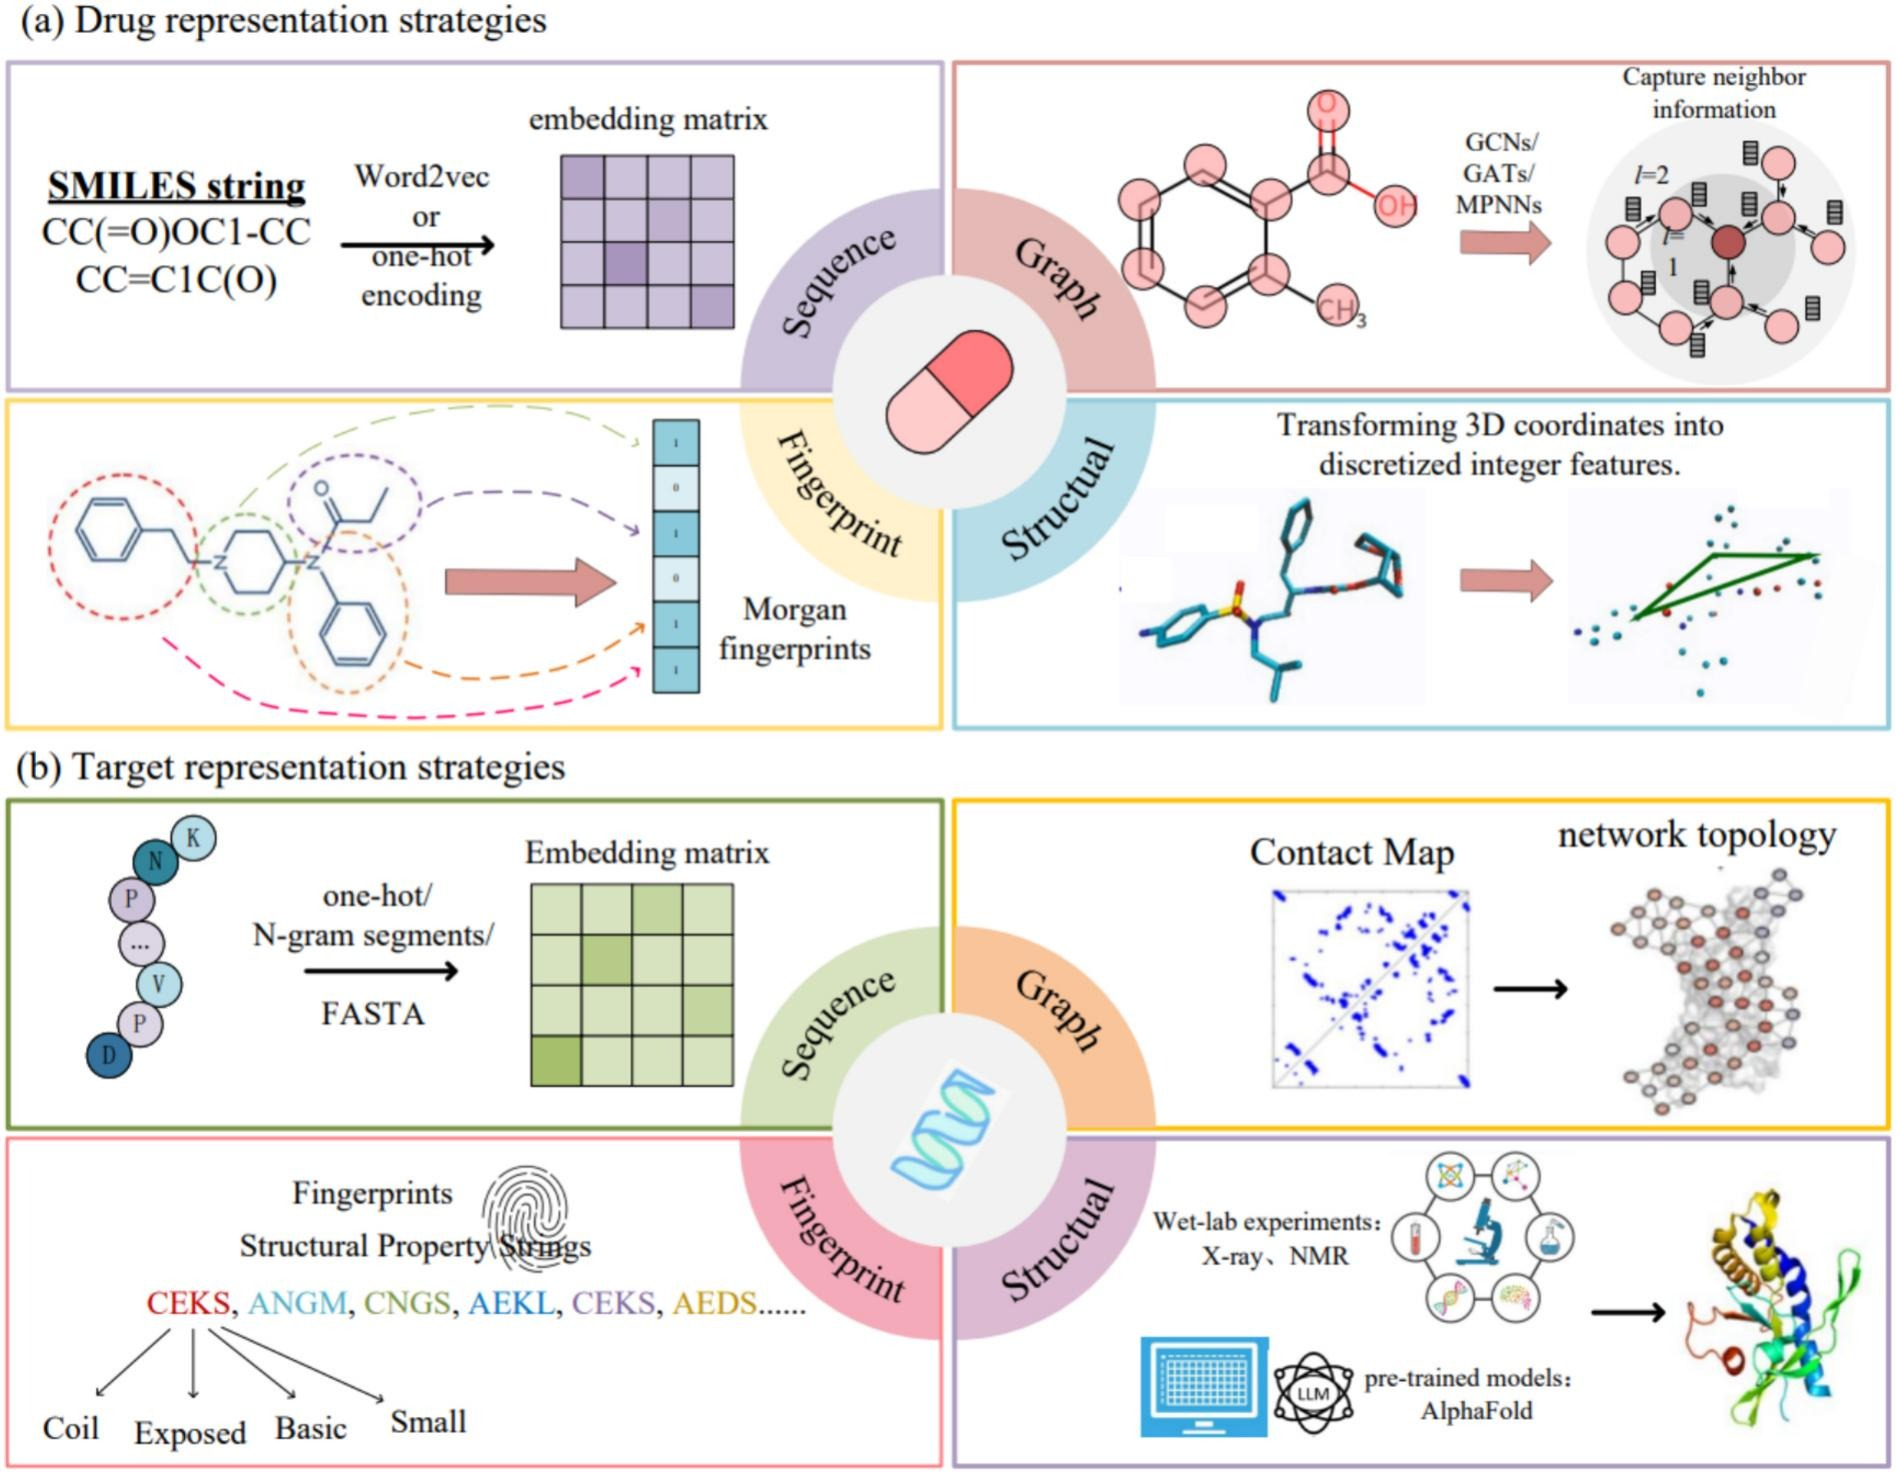
\includegraphics[width=0.75\linewidth]{figures/rappresentazioni_wang.png}
    \caption{Strategie di rappresentazione per molecole farmacologiche e proteine bersaglio. (a) Rappresentazione dei composti chimici tramite SMILES, grafi molecolari, fingerprint (Morgan) e caratteristiche strutturali 3D. \\(b) Rappresentazione dei target biologici tramite sequenze FASTA, descrittori strutturali e modelli predittivi (es. AlphaFold). Figura riprodotta con il permesso di Elsevier, da Wang et al., A unified survey on drug-target interaction and binding affinity prediction: Models, representations, and challenges", Biotechnology Advances, 2026. Licenza numero: 6286991125834.}
    \label{fig:rappresentazioni_wang}
\end{figure}
\clearpage
\section{Rappresentazioni lineari: SMILES e SELFIES}
La necessità di disporre di dati FAIR e \textit{machine readable/actionable} ha portato allo sviluppo di diverse metodologie di codifica di dati chimici in formati meno complessi, processabili da algoritmi e metodi di machine learning.
\subsection{SMILES}
Il sistema \textbf{SMILES} (Simplified Molecular-Input Line-Entry System) rappresenta lo standard moderno più diffuso per la rappresentazione di molecole chimiche nell'ambito delle applicazioni di intelligienza artificiale.\\
Si basa sulla descrizione delle strutture chimiche attraverso stringhe di caratteri alfanumerici ASCII \cite{aksamitHybridFragmentSMILESTokenization2024}, sottoponibili a processi NLP.
Una stringa SMILES rappresenta la molecola come una catena di atomi, dove le ramificazioni sono indicate tra parentesi tonde, le chiusure degli anelli da numeri corrispondenti (per esempio, 1 con 1, ecc...), i simboli "-", "=", "\#" \cite{sadeghiCanLargeLanguage2024} rappresentano diversi tipi di legame, mentre "@", "/", "\textbackslash" diverse conformazioni isomeriche \cite{aksamitHybridFragmentSMILESTokenization2024}.
$$CC(C)(C)C(=O)C(N1C=CN=C1)OC2=CC=C(C=C2)Cl$$
\begin{figure}[htbp]
    \centering
    \chemfig{C(-[::90]C)(-[::-90]C)(-[::180]C)-C(=[::90]O)-C(-[::90]N*5(-CH=N-CH=CH-))-O-P*6(-CH=CH-C(Cl)=CH-CH=)}
    \caption{Rappresentazione SMILES e struttura molecolare del Climbazolo.}
    \label{fig:climbazolo_smiles}
\end{figure}
\begin{figure}[h]
    \centering
    \begin{tikzpicture}[
        block/.style={
            rectangle, 
            draw=black, 
            thick, 
            minimum width=4.5cm, 
            minimum height=1cm, 
            align=center,
            font=\small\sffamily
        },
        textnode/.style={
            font=\small\sffamily\bfseries,
            align=center
        },
        arrow/.style={
            -{Stealth[scale=1.2]}, 
            thick
        },
        node distance=1.0cm
    ]

        \node[textnode] (smiles) {Stringa SMILES};
        
        \node[block, below=of smiles] (scomp) {1. Scomposizione};
        
        \node[block, below=of scomp] (ident) {2. Identificazione};
        
        \node[block, below=of ident] (mapp) {3. Mappatura};
        
        \node[textnode, below=of mapp] (bits) {Vettore di Bit \\ \normalfont\ttfamily[0, 1, 0, ...]};
        \draw[arrow] (smiles) -- (scomp);
        \draw[arrow] (scomp)  -- (ident);
        \draw[arrow] (ident)  -- (mapp);
        \draw[arrow] (mapp)   -- (bits);

    \end{tikzpicture}
    \caption{Flusso del processo di trasformazione chimico-digitale da stringa SMILES a vettore di bit.}
    \label{fig:smiles_to_bits_vertical}
\end{figure}
Le SMILES vengono tradotte in bit tramite \textit{processing} a Fingerprint Molecolari:
Le stringhe entrano in input per passare in una prima \textbf{Fase di Scomposizione}, da cui si ottengono frammenti di natura diversa in base all'algoritmo usato (possono essere percorsi tra atomi, aree di intorno circolare, ecc...) \cite{boldiniEffectivenessMolecularFingerprints2024}.\\
Segue poi la fase di \textbf{Encoding}, in cui ogni frammento riceve un identificatore numerico basato sulle proprietà atomiche.\\
Infine la fase di \textbf{Hashing}, dove gli identificatori vengono mappati in un vettore di bit a dimensione fissa, tramite funzioni apposite.\\  
Nonostante la sua ampia diffusione, \textbf{SMILES} presenta criticità strutturali che ne limitano l'efficacia:
\begin{itemize}
    \item Un primo limite della rappresentazione risiede nella \textbf{mancanza di univocità} che rende possibile la descrizione di una stessa molecola da molteplici stringhe diverse \cite{leonComparingSMILESSELFIES2024}.
    \item Inoltre, il sistema SMILES è soggetto a una notevole fragilità sintattica che può portare facilmente all'invalidazione delle stringe a causa di piccole mutazioni di caratteri singoli (come una parentesi non chiusa), che rendono il complesso privo di significato biologico. 
    Questa vulnerabilità risulta particolarmente problematica nell'uso di \textbf{Language Model} e modelli generativi, i quali producono combinazioni casuali di simboli durante la campionatura dello spazio latente.
    \item Infine, la natura lineare delle stringhe non premette di raffigurare correttamente la conformazione tridimensionale della molecola e le sue complesse relazioni spaziali \cite{ucakReconstructionLosslessMolecular2023}.
\end{itemize}
\subsection{SELFIES}
Le stringhe \textbf{SELFIES} (SELF-referencing Embedded Strings) sono state progettate con lo scopo di superare i limiti di SMILES, garantendo una robustezza del 100\% \cite{krennSELFIESFutureMolecular2022} ed eliminando gli errori sintattici derivati dalle variazioni di caratteri.
Ogni stringa SELFIES valida corrisponde a una molecola valida, poiché la notazione si basa su una mappatura che impedisce violazioni dei vincoli fisici e strutturali. 
A differenza di SMILES, che è una notazione descrittiva, SELFIES è più simile a una libreria di stati finiti, i quali compongono una grammatica formale, un \textbf{automa} \cite{leonComparingSMILESSELFIES2024}.\\
I SELFIES sono racchiusi tra parentesi quadre e definiscono, tramite identificatori locali, le ramificazioni e gli anelli in un unico punto, specificandone la lunghezza tramite \textit{overloading}:\\
Quando il modello incontra un token di ramificazione o di anello, i numeri immediatamente successivi vengono interpretati come dimensione della sottostruttura di riferimento \cite{leonComparingSMILESSELFIES2024}.
In questo modo vengono evitate con successo variazioni indesiderate causate da riferimenti con indici lontani tra loro nella stringa. \\
Questa prorpietà rende i SELFIES particolarmente adatti per l'impiego in modelli generativi, poiché l'intero spazio latente esplorato da questi sarebbe composto da strutture chimicamente valide, che non richiederebbero ulteriori filtri o controlli. 
\begin{figure}[htbp]
    \centering
    $$C1=CC=CC=C1$$
    $$[C][=C][C][=C][C][=C][Ring_1][=Branch_1]$$
    \caption{Confronto tra le notazioni per il benzene: SMILES (sopra) e SELFIES (sotto) \cite{krennSELFIESFutureMolecular2022}.}
    \label{fig:smiles_vs_selfies}
\end{figure}
Nonostante i vantaggi tecnici offerti dalle stringhe SELFIES in termini di robustezza, il sistema \textbf{SMILES} rimane comunque lo standard cheminformatico più popolare per diverse ragioni:\\
In particolare, la sintassi SELFIES e il suo meccanismo di overloading dei token risultano più difficili da interpretare visivamente e meno intuitivi per gli operatori umani \cite{leonComparingSMILESSELFIES2024}.
Inoltre, sorprendentemente, in alcuni task di classificazione, modelli basati su SMILES hanno mostrato di superare le controparti basate su SELFIES. Questo comportamento può essere dovuto al fatto che le SMILES, essendo più sensibili alla tokenizzazione (generano sequenze di token più brevi ed efficienti per la stessa molecola), permettono di catturare pattern unici, talvolta trascurati dai modelli SELFIES, che tendono invece a generalizzare eccessivamente le caratteristiche molecolari.\\
Questa maggiore compattezza permette ad architetture come i \textbf{Transformer} di allocare la matrice di \textbf{attention} in modo più efficace, concentrandosi su un numero minore di unità informative \cite{leonComparingSMILESSELFIES2024}.\\
\section{Fingerprint molecolari}
I \textit{fingerprint} d'altro canto adottano un approccio vettoriale:\\
Come citato prima, la molecola viene decomposta in frammenti locali che vengono poi convertiti, tramite funzioni di hashing, in un formato \textit{machine-readable}, ovvero in un vettore numerico di lunghezza fissa (di solito pari a 1024 bit).
Questi vettori codificano caratteristiche specifiche, come la presenza o l'assenza di determinate strutture (\textit{binary fingerprints}) o il numero di occorrenze di determinati pattern molecolari (\textit{count-based fingerprints}), permettendo agli algoritmi di ML di analizzare facilmente le molecole per task di \textit{Virtual Screening} e previsione di proprietà biologiche \cite{boldiniEffectivenessMolecularFingerprints2024}.\\
Esistono diverse categorie principali di fingerprint, suddivise in base al tipo di informazione che catturano \cite{boldiniEffectivenessMolecularFingerprints2024}:
\begin{itemize}
    \item Fingerprints "\textbf{String-based"}: Operano direttamente sulla stringa SMILES, frammentando la stringa in sottosequenze di dimensione fissa e calcolando il numero di occorrenze di questi frammenti.
    \item Fingerprints "\textbf{Path-based"}: Data una rappresentazione molecolare \textbf{a grafo} (che verrà approfondita nella prossima sezione), vengono analizzati i \textbf{cammini lineari}, utilizzando, ad esempio, algoritmi come il \textbf{DFS (Depth First Search)}, che percorrono la molecola partendo da ogni singolo atomo fino ad una distanza di \textit{d} legami, mantenendo un record di ogni percorso unico.
    \item Fingerprints \textbf{Farmacoforici}: Si focalizzano sulla reattività chimica piuttosto che sulla struttura. I farmacofori sono l'insieme di caratteristiche chiave di una molecola all'interno del suo ambiente biochimico, come i punti di interazione, donatori/accettori, legami a idrogeno, gruppi idrofobici, ecc...
    Questi fingerprints codificano il modo in cui la molecola interagisce con l'ambiente circostante, concentrandosi maggiormente sulle proprietà funzionali, piuttosto che sulla struttura anatomica esatta.
    \item Fingerprints "\textbf{Substructure-based}": Basati sulla presenza di sottostrutture chimiche predefinite. Questo tipo di fingerprints utilizza un "dizionario" di frammenti noti, precedentemente individuati da esperti.
    \item Fingerprints \textbf{Circolari}: Partendo da un atomo, l'algoritmo di fingerptint aggrega le informazioni degli atomi vicini tra loro entro un raggio crescente, di fatto scomponendo la molecola in frammenti sullo stesso arco.
    Si tratta della tecnica più utilizzata per i modelli di Machine Learning, poiché è in grado di catturare informazioni sull'ambiente locale dell'atomo in modo strutturato ed esaustivo.
\end{itemize}
\subsection{Esempi di fingerprints}
Alcuni esempi appartenenti alla categoria di rappresentazione con \textbf{fingerprint molecolari} sono le \textbf{Morgan fingerprints} (o \textit{Extended Connectivity Fingerprints} (ECFP)) e le \textbf{MACCS key}.\\
Le prime si distinguono come strumento fondamentale e standard \textit{de facto} per la codifica dei composti farmaceutici \textit{drug-like}. 
\\Queste fingerprints \textbf{circolari}, con lunghezza pari a $1024$ bit, sono in grado di costruire dinamicamente i frammenti delle sottostrutture molecolari, a partire dalla loro rappresentazione a grafo \cite{boldiniEffectivenessMolecularFingerprints2024}.\\
Le \textbf{MACCS key (Molecular Access System)}, invece, si basano su un approccio più storico e utilizzano, come suggerito dal nome, un \textbf{dizionario} statico predefinito di sottostrutture, da cui attingere per codificare le strutture:\\
Sono rappresentate da un vettore binario da \textbf{166} bit di lunghezza. Ognuno di questi bit codifica la assenza/presenza ({0,1}) di una specifica caratteristica strutturale, definita tramite i pattern \textbf{SMARTS} (SMILES Arbitrary Target 
Specification) \cite{boldiniEffectivenessMolecularFingerprints2024} \cite{ucakReconstructionLosslessMolecular2023} che identificano, all'interno del dizionario, frammenti, gruppi funzionali o motivi molecolari.
\begin{lstlisting}[language=Python, caption={Estrazione delle MACCS Keys tramite RDKit}, label={lst:maccs_code}]
    from rdkit import Chem
    from rdkit.Chem import MACCSkeys

    smiles = "CC(C)Cc1ccc(cc1)C(C)C(=O)O"
    mol = Chem.MolFromSmiles(smiles)
    maccs_key = MACCSkeys.GenMACCSKeys(mol)
    bit_string = maccs_key.ToBitString()

    maccs_166 = [int(b) for b in bit_string][1:]
\end{lstlisting}
\begin{figure}
    \centering
    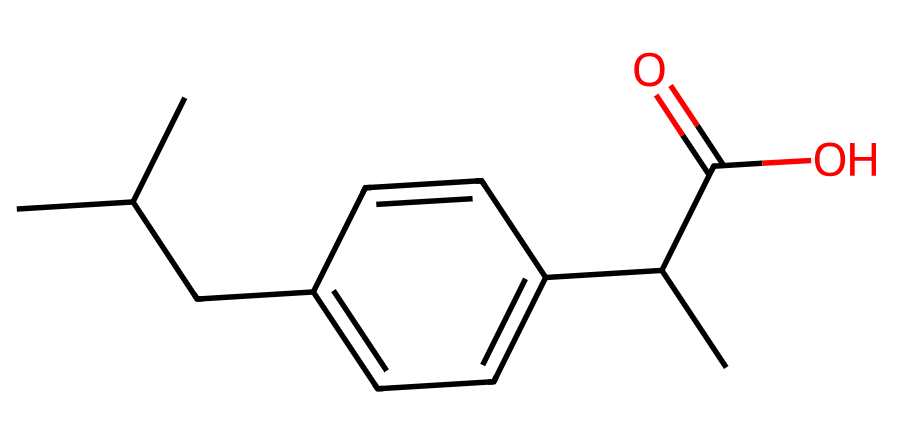
\includegraphics[width=0.5\linewidth]{figures/svgIbuprofene.png}
    \caption{Struttura chimica dell'Ibuprofene. \\Indici dei bit attivi rilevati: [74, 115, 123, 139, 141, 149, 154, 155, 157, 159, 160, 162, 163, 164, 165]}
\end{figure}
\begin{figure}
    \centering
    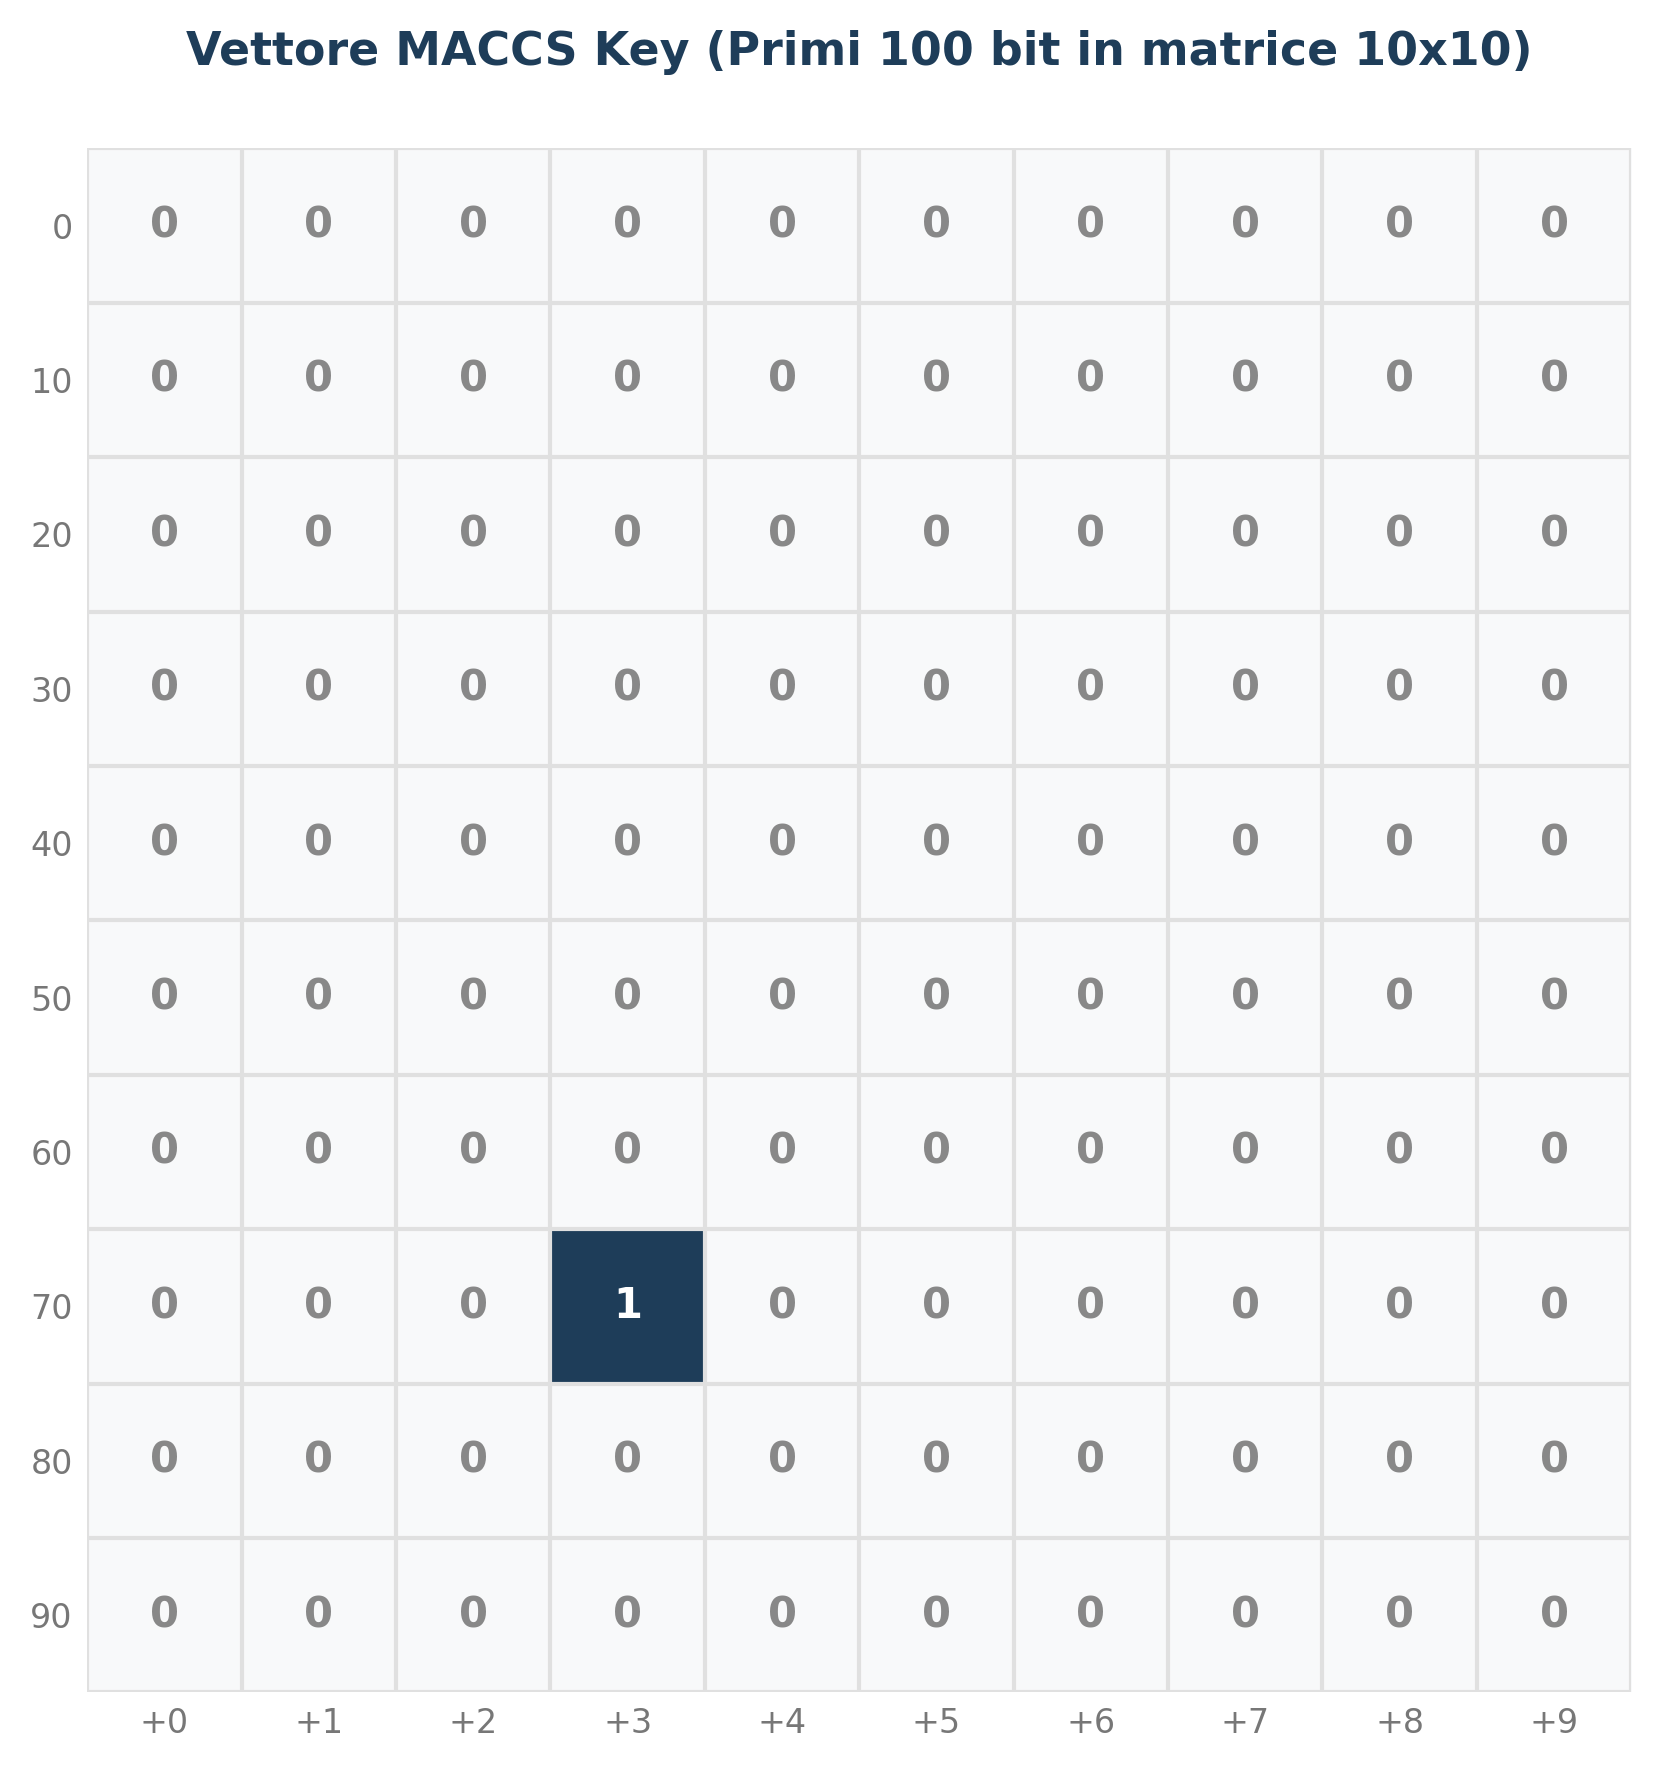
\includegraphics[width=0.4\linewidth]{figures/vettore_maccs_ibu.png}
    \caption{Primi 100 bit del fingerprint dell'Ibuprofene}
\end{figure}
Nonostante i fingerprint molecolari offrano diversi vantaggi significativi rispetto alle rappresentazioni lineari, specialmente in termini di efficienza computazionale e interpretabilità, questi presentano una perdita di informazioni non trascurabile durante il loro processo di codifica \textit{hashing}, soprattutto per quanto riguarda i dati sulla connettività dei frammenti \cite{ucakReconstructionLosslessMolecular2023}.
È quindi necessario risalire a una \textbf{ricostruzione lossless} (senza perdita di informazioni), invertendo la traduzione dei fingerprint.
Si tratta di un processo computazionale basato sull'architettura \textbf{Transformer}, che viene utilizzata come un sistema di traduzione in grado di apprendere le dipendenze globali tra input (i bit del fingerprint) e output (token di stringhe molecolari molecolare), grazie al meccanismo di \textit{multi-head attention}.
Il modello riesce quindi a decodificare i fingerprint strutturali riconducendoli a rappresentazioni lineari (SMILES o SELFIES) \cite{ucakReconstructionLosslessMolecular2023}.\\
\section{Rappresentazione a grafo}
La rappresentazione a \textbf{grafo} contituisce l'approccio più intuitivo e fedele alla realtà fisica per la digitalizzazione delle strutture chimiche, superando i limiti informativi delle notazioni lineari e minimizzando la perdita di dati.\\
La molecola viene rappresentata come un grafo non orientato  $G=(V,E)$ \cite{wangGraphNeuralNetworks2023}, in cui:
\begin{description}
    \item[$V$ (Nodi):] Rappresentano gli atomi della molecola. 
    \item[$E$ (Archi):] Rappresentano i legami chimici interatomici.
\end{description}
Tale struttura permette di codificare direttamente la topologia (informazioni bidimensionali, come i legami covalenti) e la connettività della molecola (la geometria, le informazioni tridimensionali), trasformando le proprietà del composto in \textbf{matrici} elaborabili da modelli di Intelligenza Artificiale.\\
Per essere interpretata dai computer, la struttura del grafo viene convertita in matrici, convertendo così la informazioni chimiche in un linguaggio matematico adatto ad essere appreso dai modelli \cite{wangGraphNeuralNetworks2025}.\\
Questa rappresentazione è il pilastro fondamentale per le \textbf{GNN (Graph Neural Networks)}, argomento che verrà affrontato nel prossimo capitolo.
\begin{figure}
    \centering
    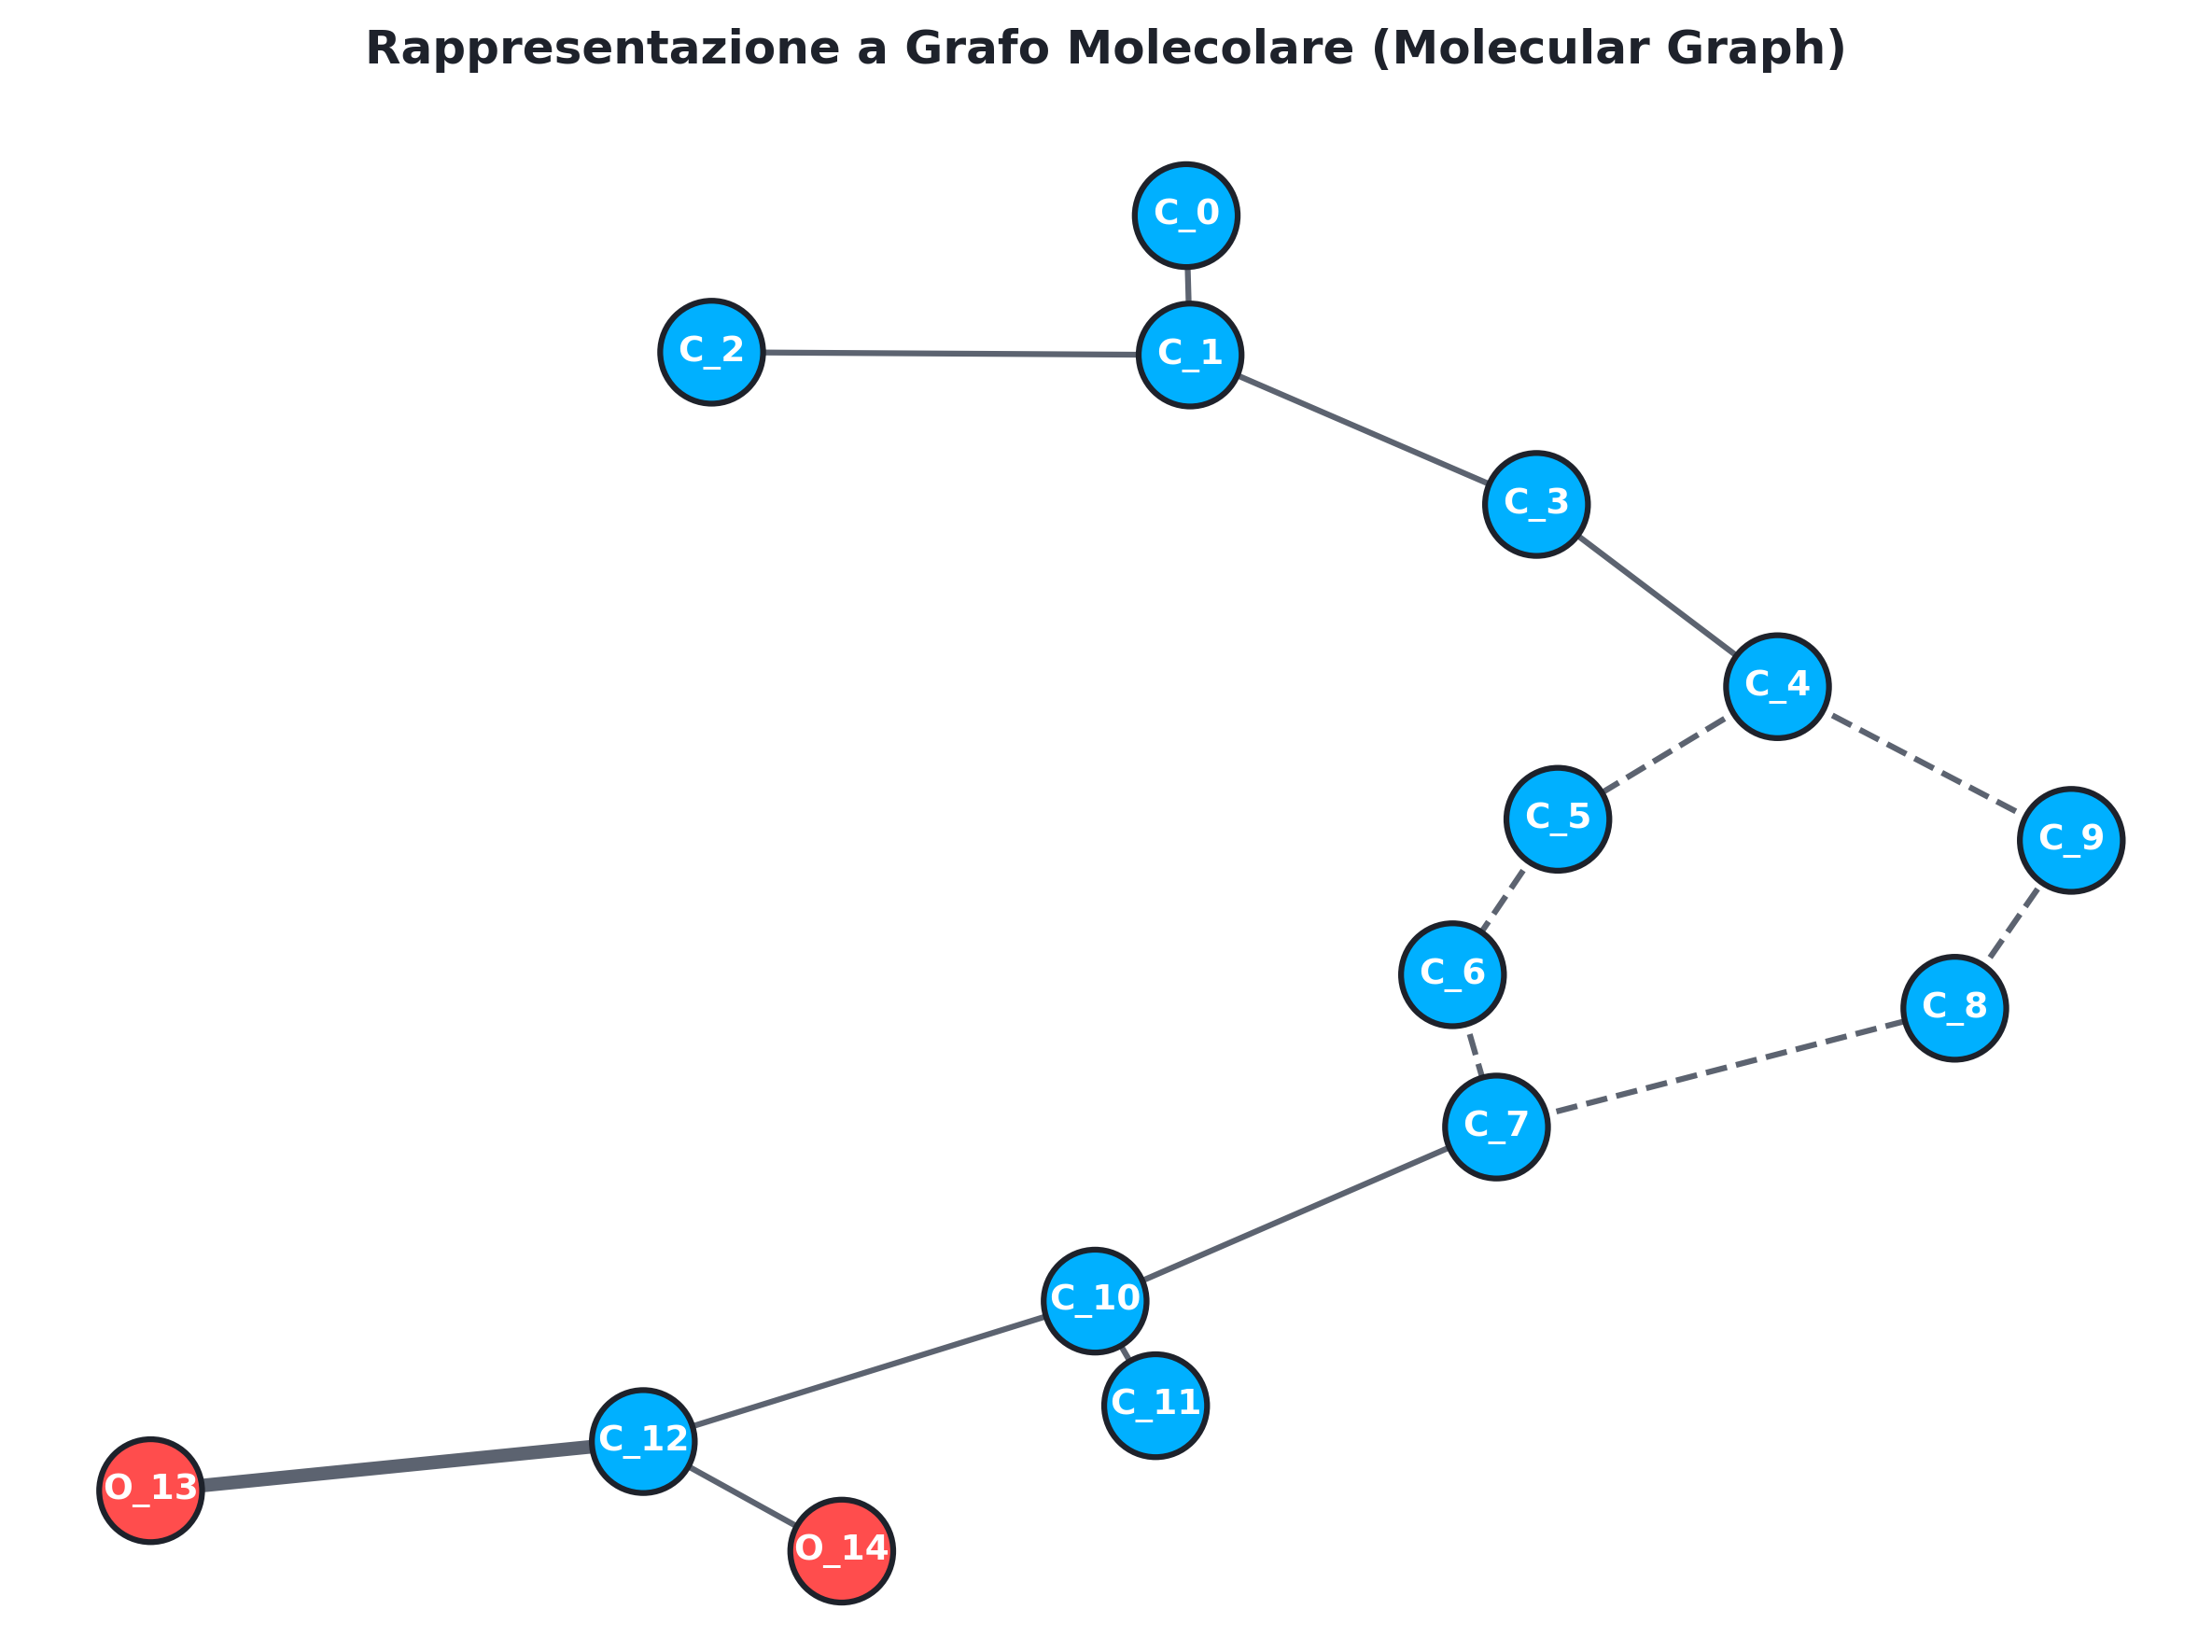
\includegraphics[width=0.75\linewidth]{figures/molecular_graph_ibu.png}
    \caption{Rappresentazione topologica non orientata $G = (V, E)$ dell'Ibuprofene generata da codice grazie a librerie RDKit e NetworkX.}
    \label{fig:graph}
\end{figure}
\clearpage
\section{Embedding molecolari e modelli pre-addestrati}
L'\textbf{embedding molecolare} è un'operazione fondamentale nella ricerca farmaceutica.
Questo processo consiste nel trasformare le informazioni relative al contesto strutturale e chimico di una molecola in una \textbf{rappresentazione numerica}, tipicamente sotto forma di vettori densi ad alta dimensione.\\
Questa pratica si basa sulla seguente ipotesi: \textbf{tutte le molecole strutturalmente simili, presentano comportamenti e proprietà altrettanto simili}.  Seguendo questa ipotesi, l'embeddig cerca di mappare queste molecole in punti vicini nello spazio vettoriale \cite{sadeghiCanLargeLanguage2024}.\\
I vettori di embedding possono essere generati principalmente in due modi distinti:
\begin{itemize}
    \item \textbf{Embedding basati su Grafi} (come ad esempio i \textbf{GNN}). Gli embedding vengono estratti dalla struttura a grafo tramite le fasi di \textit{update} dei nodi-atomo e di \textit{message passing} \cite{wangEvaluatingSelfSupervisedLearning2023}.
    In particolare, per ogni atomo $u$, viene calcolato l'embedding $h_u^{(t+1)}$ (con $t$ che rappresenta il livello corrente del \textit{message passing}) aggregando i messaggi dai nodi vicini $v$. Durante il passaggio dei messaggi vengono inoltre integrate le caratteristiche dei legami chimici rappresentati dagli archi della GNN, $x_{uv}$.
    Durante la fase di \textit{readout}, gli embedding di tutti i nodi vengono aggregati. Il risultato è un vettore riassuntivo degli embedding molto ricchi calcolati nei vari livelli della rete, che sarà usato per compiere predizione sulla molecola nel suo complesso, integrando le informazioni sulle sottostrutture e la sua topologia.
    \item \textbf{Embedding basati su stringhe (LLM)}. Sfruttano le rappresentazioni lineari testuali come \textbf{SMILES} per effettuare la codifica in vettori, catturando le informazioni semantiche e contestuali \cite{sadeghiCanLargeLanguage2024}. Questo processo avviene tramite tokenizzazione delle stringhe SMILES da parte di \textbf{Large Language Models} (che sono in grado di processarle in quanto dati in formato testuale), che vengono quindi elaborati dall'architettura a \textbf{Transformer}.
\end{itemize}
Per verificare la qualità dell'embedding estratto si utilizzano i \textbf{modelli di probe}, ovvero semplici classificatori lineari addestrati su vettori fissi, che sono in grado di verificare le informazioni catturate.\\
Un embedding di alta qualità dovrebbe essere in grado di rappresentare correttamente \textbf{proprietà topologiche}, \textbf{proprietà nello spazio} e \textbf{sottostrutture molecolari}.
\section{Rappresentazione delle proteine target: FASTA}
Oltre alle piccole molecole, è necessario anche rappresentare in modo corretto le sequenze amminoacidiche che compongono i target terapeutici.\\
Lo standard \textbf{FASTA} è un formato testuale ampiamente utilizzato per questo task.
La struttura primaria della proteina viene codificata come una stringa lineare di caratteri simbolici in cui ogni lettera corrisponde a un amminoacido specifico \cite{wangUnifiedSurveyDrugtarget2026a}.
Essendo unidimensionale però, questo formato di rappresentazione non è adatto a cogliere gli aspetti più importanti delle sequenze proteiche, ovvero la loro conformazione tridimensionale.\\
Nel contesto dell'analisi sequence-based, la stringa in formato FASTA rappresenta l'input standard per i modelli predittivi di Deep Learning, come vedremo nei capitoli successivi.
\clearpage
\begin{lstlisting}[caption={Sequenza FASTA ufficiale della proteina CFTR (Cystic fibrosis transmembrane conductance regulator) umana (UniProt P13569).}, label={lst:fasta_cox2}]
>sp|P13569|CFTR_HUMAN Cystic fibrosis transmembrane conductance regulator OS=Homo sapiens OX=9606 GN=CFTR PE=1 SV=3
MQRSPLEKASVVSKLFFSWTRPILRKGYRQRLELSDIYQIPSVDSADNLSEKLEREWDRE
LASKKNPKLINALRRCFFWRFMFYGIFLYLGEVTKAVQPLLLGRIIASYDPDNKEERSIA
IYLGIGLCLLFIVRTLLLHPAIFGLHHIGMQMRIAMFSLIYKKTLKLSSRVLDKISIGQL
VSLLSNNLNKFDEGLALAHFVWIAPLQVALLMGLIWELLQASAFCGLGFLIVLALFQAGL
GRMMMKYRDQRAGKISERLVITSEMIENIQSVKAYCWEEAMEKMIENLRQTELKLTRKAA
YVRYFNSSAFFFSGFFVVFLSVLPYALIKGIILRKIFTTISFCIVLRMAVTRQFPWAVQT
WYDSLGAINKIQDFLQKQEYKTLEYNLTTTEVVMENVTAFWEEGFGELFEKAKQNNNNRK
TSNGDDSLFFSNFSLLGTPVLKDINFKIERGQLLAVAGSTGAGKTSLLMVIMGELEPSEG
KIKHSGRISFCSQFSWIMPGTIKENIIFGVSYDEYRYRSVIKACQLEEDISKFAEKDNIV
LGEGGITLSGGQRARISLARAVYKDADLYLLDSPFGYLDVLTEKEIFESCVCKLMANKTR
ILVTSKMEHLKKADKILILHEGSSYFYGTFSELQNLQPDFSSKLMGCDSFDQFSAERRNS
ILTETLHRFSLEGDAPVSWTETKKQSFKQTGEFGEKRKNSILNPINSIRKFSIVQKTPLQ
MNGIEEDSDEPLERRLSLVPDSEQGEAILPRISVISTGPTLQARRRQSVLNLMTHSVNQG
QNIHRKTTASTRKVSLAPQANLTELDIYSRRLSQETGLEISEEINEEDLKECFFDDMESI
PAVTTWNTYLRYITVHKSLIFVLIWCLVIFLAEVAASLVVLWLLGNTPLQDKGNSTHSRN
NSYAVIITSTSSYYVFYIYVGVADTLLAMGFFRGLPLVHTLITVSKILHHKMLHSVLQAP
MSTLNTLKAGGILNRFSKDIAILDDLLPLTIFDFIQLLLIVIGAIAVVAVLQPYIFVATV
PVIVAFIMLRAYFLQTSQQLKQLESEGRSPIFTHLVTSLKGLWTLRAFGRQPYFETLFHK
ALNLHTANWFLYLSTLRWFQMRIEMIFVIFFIAVTFISILTTGEGEGRVGIILTLAMNIM
STLQWAVNSSIDVDSLMRSVSRVFKFIDMPTEGKPTKSTKPYKNGQLSKVMIIENSHVKK
DDIWPSGGQMTVKDLTAKYTEGGNAILENISFSISPGQRVGLLGRTGSGKSTLLSAFLRL
LNTEGEIQIDGVSWDSITLQQWRKAFGVIPQKVFIFSGTFRKNLDPYEQWSDQEIWKVAD
EVGLRSVIEQFPGKLDFVLVDGGCVLSHGHKQLMCLARSVLSKAKILLLDEPSAHLDPVT
YQIIRRTLKQAFADCTVILCEHRIEAMLECQQFLVIEENKVRQYDSIQKLLNERSLFRQA
ISPSDRVKLFPHRNSSKCKSKPQIAALKEETEEEVQDTRL
\end{lstlisting}
\subsection{AlphaFold}
La rappresentazione unidimensionale delle sequenze amminoacidiche non è sufficiente a spiegare in modo esaustivo la conformazione e il ripiegamento tridimensionale delle proteine target.\\
Queste proprietà strutturali sono essenziali per capire al meglio le caratteristiche e i siti di legame del bersaglio, e si rende quindi necessario l'utilizzo di tools in grado di predirle.\\
Uno di questi strumenti è proprio \textbf{AlphaFold}, citata nel capitolo di introduzione come uno dei casi più eclatanti di un dialogo di successo tra informatica e biochimica:\\
Viene sfruttata un'architettura a rete neurale per integrare le nozioni chimico-fisiche e biologiche all'interno dell'insieme di regole di conformazione delle proteine.
La rete prende in input una sequenza FASTA e la processa per ricercare le zone con avvolgimento più alto, le quali determinano la complessità della struttura.\\
Il modello si divide in due fasi principali:
\begin{enumerate}
    \item \textbf{Evoformer:} Primo modulo incaricato della previsione della struttura. Si approccia al problema computazionale interpretandolo come un \textbf{problema di inferenza di grafi} nello spazio tridimensionale. Tiene traccia degli amminoacidi propensi a mutare insieme, e a creare quindi strutture di avvolgimento complesse, tramite \textbf{Multiple Sequence Alignments} o \textbf{MSA}. Queste sono collezioni di sequenze di proteine omologhe allineate tra loro in un array bidimensionale, la cui analisi risulta utile per la previsone di coordinazioni tra amminoacidi e siti di ripiegamento proteico \cite{jumperHighlyAccurateProtein2021}.
    \item \textbf{Modello di Struttura:} Trasforma le informazioni ricavate dall'Evoformer in coordinate 3D reali. Ogni amminoacido è trattato come un corpo rigido indipendente, o "residue gas", che può ruotare e traslare nello spazio fino ad assumere la sua posizione "corretta" all'interno della conformazione della catena proteica.
    Viene usato un meccanismo di \textbf{Attenzione} (\textbf{Invariant Point Attention, o IPA}) le cui iterazioni raffinano le informazioni spaziali degli elementi.
\end{enumerate}
\begin{figure}
    \centering
    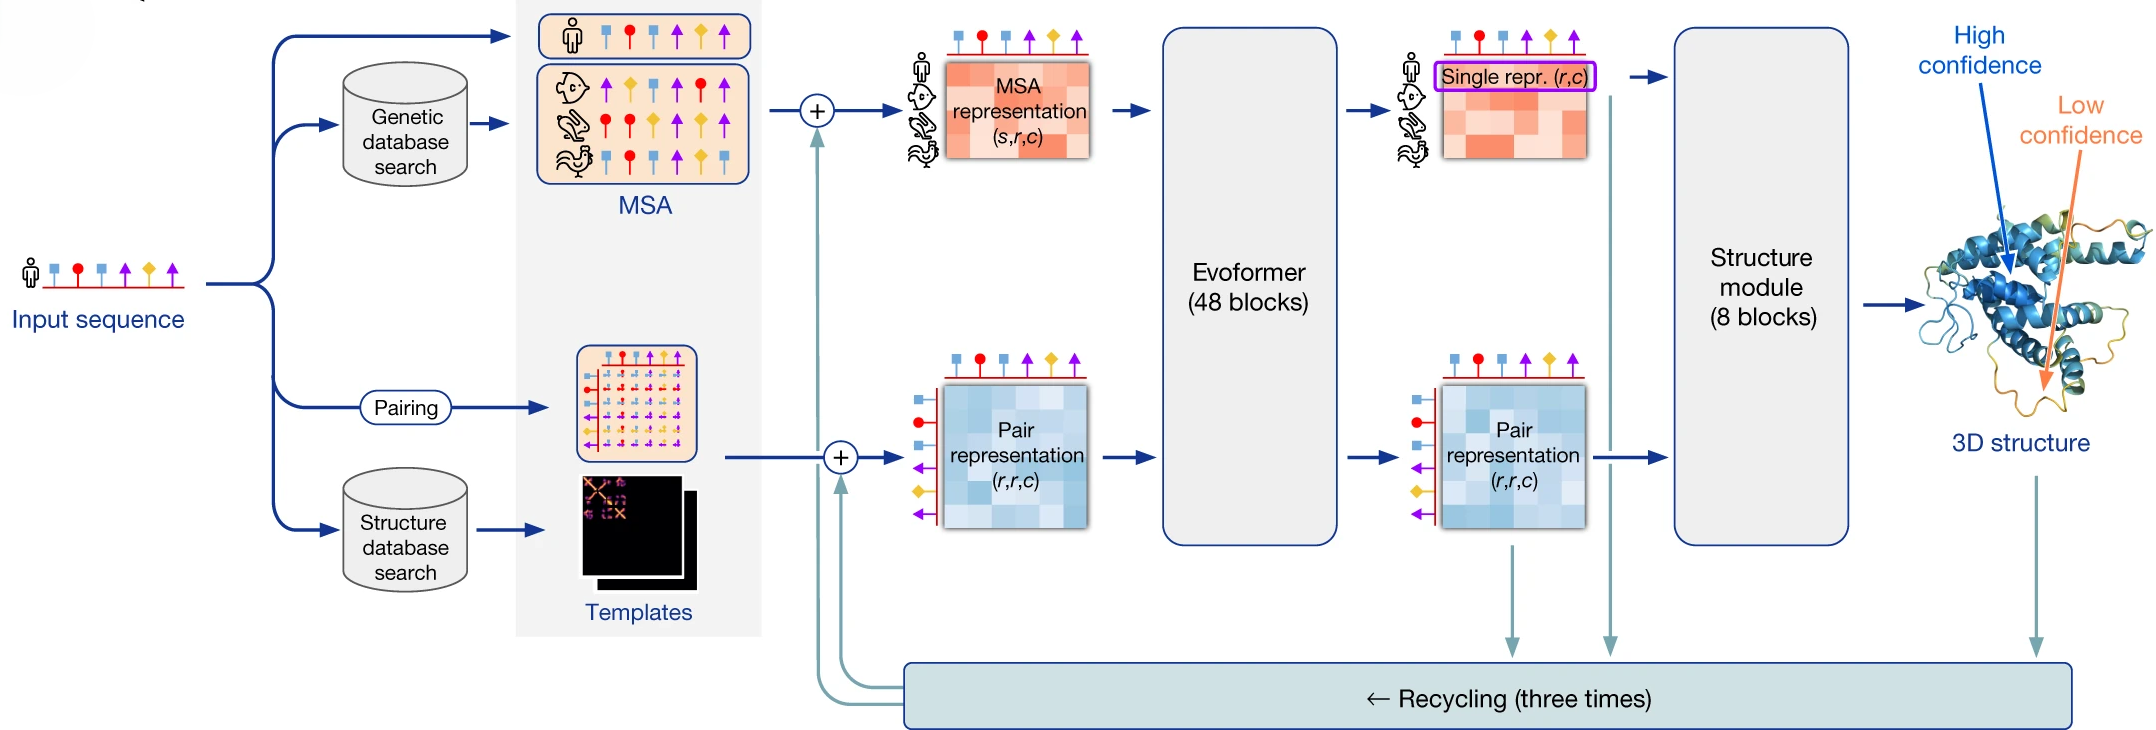
\includegraphics[width=1\linewidth]{figures/alphafold_pipeline.png}
    \caption{Schema semplificato della rete neurale di AlphaFold. Adattato e modificato dall'opera originale di Jumper et al. (2021), disponibile in Open Access sotto licenza Creative Commons Attribution 4.0 International (\url{http://creativecommons.org/licenses/by/4.0/}).}
    \label{fig:alphafold}
\end{figure}





